\documentclass[12pt, letterpaper]{article}
\usepackage{graphicx}
\usepackage[margin=1in]{geometry}
\usepackage{amsmath, amssymb, amsthm, mathrsfs}
\usepackage{fancyhdr}
\usepackage{tikz}
\usepackage{enumerate}
\usepackage{cancel}
\usetikzlibrary{positioning}
\usepackage[utf8]{inputenc}
\usepackage{xcolor}
\usepackage{framed}
\title{HW 1.3}
\author{Your Name}
\date{\today}
\pagestyle{fancy}
\renewcommand{\headrulewidth}{0pt}
\renewcommand{\footrulewidth}{0pt}
\fancyhf{}
\rhead{
    Zack Abdirashid\\
    3/19/26 \\
    MATH 405
}
\rfoot{Page \thepage}
\begin{document}
\paragraph{\underline{2.3} \\ \\} 
\textbf{1.}(r) Find the chromatic number of the following graph 
\begin{center}
   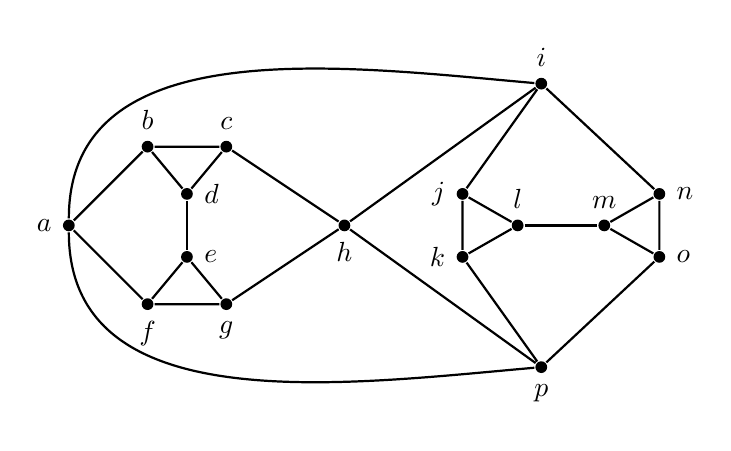
\begin{tikzpicture}[
    dot/.style={circle, fill, inner sep=1.5pt},
    thick
]

  % --- LEFT SECTION ---
  \node[dot, label=left:$a$] (a) at (0,0) {};
  \node[dot, label=above:$b$] (b) at (1,1) {};
  \node[dot, label=above:$c$] (c) at (2,1) {};
  \node[dot, label=right:$d$] (d) at (1.5,0.4) {};
  \node[dot, label=right:$e$] (e) at (1.5,-0.4) {};
  \node[dot, label=below:$f$] (f) at (1,-1) {};
  \node[dot, label=below:$g$] (g) at (2,-1) {};
  
  % --- CENTER JUNCTION ---
  \node[dot, label=below:$h$] (h) at (3.5,0) {};

  % --- RIGHT SECTION ---
  \node[dot, label=above:$i$] (i) at (6,1.8) {};
  \node[dot, label=left:$j$] (j) at (5,0.4) {};
  \node[dot, label=left:$k$] (k) at (5,-0.4) {};
  \node[dot, label=above:$l$] (l) at (5.7,0) {};
  \node[dot, label=above:$m$] (m) at (6.8,0) {};
  \node[dot, label=right:$n$] (n) at (7.5,0.4) {};
  \node[dot, label=right:$o$] (o) at (7.5,-0.4) {};
  \node[dot, label=below:$p$] (p) at (6,-1.8) {};

  % --- DRAWING EDGES ---

  % Left shape connections
  \draw (a) -- (b) -- (c) -- (h);
  \draw (a) -- (f) -- (g) -- (h);
  \draw (b) -- (d) -- (c);
  \draw (f) -- (e) -- (g);
  \draw (d) -- (e);

  % Right shape connections
  \draw (h) -- (i) -- (j) -- (k) -- (p) -- (h);
  \draw (i) -- (n) -- (o) -- (p);
  \draw (j) -- (l) -- (k);
  \draw (n) -- (m) -- (o);
  \draw (l) -- (m);

  % Outer curved arcs
  \draw (a) to[out=90, in=175] (i);
  \draw (a) to[out=-90, in=-175] (p);

\end{tikzpicture} \\
* \text{$\chi(G) \geq 3$ b/c a $K_3$ is contained in the graph}
\end{center} \\
\begin{center}
   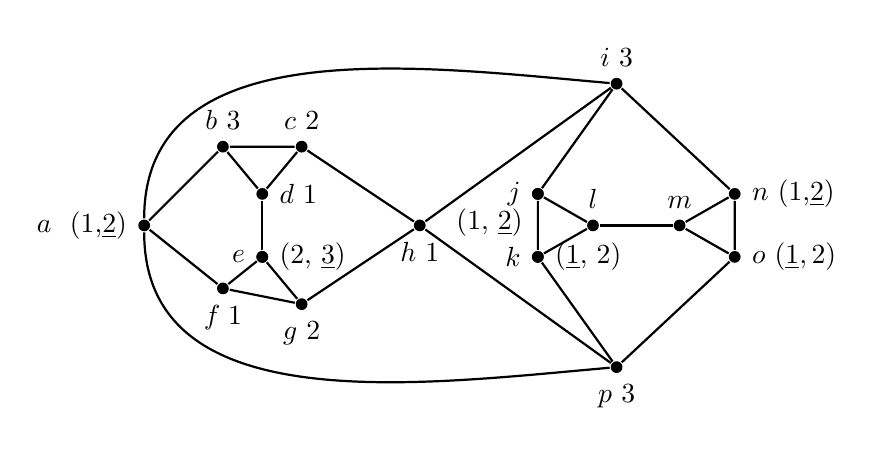
\begin{tikzpicture}[
    dot/.style={circle, fill, inner sep=1.5pt},
    thick
]

  % --- LEFT SECTION ---
  \node[dot, label=left:$\text{$a$ \ (1,\underline{2})}$] (a) at (0,0) {};
  \node[dot, label=above:$b \ 3$] (b) at (1,1) {};
  \node[dot, label=above:$c \ 2$] (c) at (2,1) {};
  \node[dot, label=right:$d \ 1$] (d) at (1.5,0.4) {};
  \node[dot, label=left:$e$] (e) at (1.5,-0.4) {};
  \node[dot, label=right:$\text{(2, \underline{3})}$] (e) at (1.5,-0.4) {};
  \node[dot, label=below:$f \; \text{1}$] (f) at (1,-0.8) {};
  \node[dot, label=below:$g \ 2$] (g) at (2,-1) {};
  
  % --- CENTER JUNCTION ---
  \node[dot, label=below:$h \ 1$] (h) at (3.5,0) {};

  % --- RIGHT SECTION ---
  \node[dot, label=above:$i \ 3$] (i) at (6,1.8) {};
  \node[dot, label=left:$j$] (j) at (5,0.4) {};
  \node[dot, label=below left:$\text{(1, \underline{2})}$] (j) at (5,0.4) {};
  \node[dot, label=left:$k$] (k) at (5,-0.4) {};
  \node[dot, label= right:$\text{(\underline{1}, 2)}$] (k) at (5,-0.4) {};
  \node[dot, label=above:$l$] (l) at (5.7,0) {};
  \node[dot, label=above:$m$] (m) at (6.8,0) {};
  \node[dot, label=right:$\text{$n$ (1,\underline{2})}$] (n) at (7.5,0.4) {};
  \node[dot, label=right:$\text{$o \ (\underline{1}, 2$)}$] (o) at (7.5,-0.4) {};
  \node[dot, label=below:$p \ 3$] (p) at (6,-1.8) {};

  % --- DRAWING EDGES ---

  % Left shape connections
  \draw (a) -- (b) -- (c) -- (h);
  \draw (a) -- (f) -- (g) -- (h);
  \draw (b) -- (d) -- (c);
  \draw (f) -- (e) -- (g);
  \draw (d) -- (e);

  % Right shape connections
  \draw (h) -- (i) -- (j) -- (k) -- (p) -- (h);
  \draw (i) -- (n) -- (o) -- (p);
  \draw (j) -- (l) -- (k);
  \draw (n) -- (m) -- (o);
  \draw (l) -- (m);

  % Outer curved arcs
  \draw (a) to[out=90, in=175] (i);
  \draw (a) to[out=-90, in=-175] (p);
\end{tikzpicture}
\begin{align*}
    &- \text{WLOG color $d, c, b$ by $1,2,3$} \\
&- \textbf{Choose $e: 3, \ a : 2$} \\
&\quad - \textbf{Force $f: 1, \ g: 2$} \\
&\quad\quad - \textbf{Choose $h:1$} \\
&\quad\quad - \textbf{Force $i, p: 3$} \\
&\quad\quad - \textbf{Choose $n,j:2$} \ \text {and $o, k: 1$}  \\
&\quad\quad  - \text{Cannot be done because $l$ is adjacent to $m$ and both are adjacent to a 1 and 2, l or m: 4} \\
&\quad-\textbf{Backtrack}\ \text{to $h:1$, \textbf{Force} $h: 3$} \\
&\quad\quad\quad\text{Cannot be done because $l \ \text{or} \ m$ are still  forced to be 4} \\
& - \textbf{Backtrack} \ \text{to $e:3, \ a:2$, \textbf{Force} \ $a:1, e:2$} \\
&\quad- \text{Cannot be done because $l \ \text{or} \ m$ are still forced to be 4}  \\ \\
\end{align*}
\end{center}
\begin{center}
    \Rightarrow \ \text{$\chi(G) \geq 4$} \\
    \begin{center}
        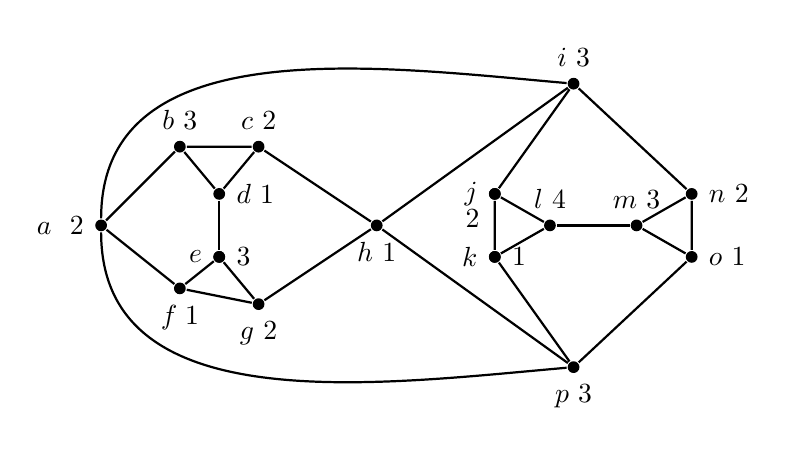
\begin{tikzpicture}[
    dot/.style={circle, fill, inner sep=1.5pt},
    thick
]

  % --- LEFT SECTION ---
  \node[dot, label=left:$\text{$a$ \ 2}$] (a) at (0,0) {};
  \node[dot, label=above:$b \ 3$] (b) at (1,1) {};
  \node[dot, label=above:$c \ 2$] (c) at (2,1) {};
  \node[dot, label=right:$d \ 1$] (d) at (1.5,0.4) {};
  \node[dot, label=left:$e$] (e) at (1.5,-0.4) {};
  \node[dot, label=right:$\text{3}$] (e) at (1.5,-0.4) {};
  \node[dot, label=below:$f \; \text{1}$] (f) at (1,-0.8) {};
  \node[dot, label=below:$g \ 2$] (g) at (2,-1) {};
  
  % --- CENTER JUNCTION ---
  \node[dot, label=below:$h \ 1$] (h) at (3.5,0) {};

  % --- RIGHT SECTION ---
  \node[dot, label=above:$i \ 3$] (i) at (6,1.8) {};
  \node[dot, label=left:$j$] (j) at (5,0.4) {};
  \node[dot, label=below left:$\text{2}$] (j) at (5,0.4) {};
  \node[dot, label=left:$k$] (k) at (5,-0.4) {};
  \node[dot, label= right:$\text{1}$] (k) at (5,-0.4) {};
  \node[dot, label=above:$l \ 4$] (l) at (5.7,0) {};
  \node[dot, label=above:$m \ 3$] (m) at (6.8,0) {};
  \node[dot, label=right:$\text{$n$ 2}$] (n) at (7.5,0.4) {};
  \node[dot, label=right:$\text{$o \ 1$}$] (o) at (7.5,-0.4) {};
  \node[dot, label=below:$p \ 3$] (p) at (6,-1.8) {};

  % --- DRAWING EDGES ---

  % Left shape connections
  \draw (a) -- (b) -- (c) -- (h);
  \draw (a) -- (f) -- (g) -- (h);
  \draw (b) -- (d) -- (c);
  \draw (f) -- (e) -- (g);
  \draw (d) -- (e);

  % Right shape connections
  \draw (h) -- (i) -- (j) -- (k) -- (p) -- (h);
  \draw (i) -- (n) -- (o) -- (p);
  \draw (j) -- (l) -- (k);
  \draw (n) -- (m) -- (o);
  \draw (l) -- (m);

  % Outer curved arcs
  \draw (a) to[out=90, in=175] (i);
  \draw (a) to[out=-90, in=-175] (p);
\end{tikzpicture}
    \end{center} \\
    \Rightarrow \ \boxed{$\chi(G) = 4$}
\end{center}
\end{document}